\documentclass{article}
\usepackage[utf8]{inputenc}
%\usepackage{geometry}
\usepackage{amsmath}
\usepackage{booktabs}
\usepackage{longtable}
\usepackage{array}
\usepackage{graphicx}
\usepackage{float}
\usepackage{xcolor}
\usepackage{pgfplots}
\usepackage{siunitx}
\usepackage{hyperref}
\usepackage{caption}
\pgfplotsset{compat=1.15}

\input{/Users/rhoge/TeX/00.3_Headers/doc_headers.tex} % Common preamble stuff shared in all sections
\usepackage[yyyymmdd,hhmmss]{datetime}
\fancyhead[R]{}
\fancyfoot[C]{[\today\ \currenttime]}
\fancyhead[C]{\textit{\small DRAFT}}

\geometry{margin=1in}

\title{Analysis of Montreal's Parametric Budget Model for Borough Transfers\\
\large 2017-2022}
\author{}
\date{\today}

\begin{document}

\maketitle

\tableofcontents

\section{Introduction}

The City of Montreal employs a parametric budget model to determine the annual budget transfers to its various boroughs. This document analyzes this model as implemented in the MATLAB script, focusing particularly on how it applies to the borough of Côte-des-Neiges–Notre-Dame-de-Grâce (CDN-NDG). The analysis also examines the relationship between borough-specific tax revenues and the central transfers received, and offers comparisons between CDN-NDG, Saint-Laurent, and Sud-Ouest boroughs.

The parametric model considered here covers the fiscal years 2017 through 2022. It calculates budget transfers based on numerous parameters including demographic data, geographic characteristics, and specific fiscal adjustments that vary by borough and by year.

\section{General Structure of the Parametric Budget Model}

The parametric budget model can be conceptualized as a multi-step process that begins with the previous year's budget and applies various adjustments and parameters to determine the next year's budget. This process is repeated annually, with each year building upon the results of the previous year.

\subsection{Basic Mathematical Framework}

The general formula for calculating a given year's budget transfer can be expressed as:

\begin{equation}
T_y = T_{y-1} + I_y + A_y + P_y
\end{equation}

Where:
\begin{itemize}
    \item $T_y$ is the total transfer for year $y$
    \item $T_{y-1}$ is the previous year's transfer
    \item $I_y$ represents indexation adjustments
    \item $A_y$ represents various parametric adjustments
    \item $P_y$ represents post-transfer adjustments
\end{itemize}

The parametric adjustments ($A_y$) encompass multiple components, including:

\begin{equation}
A_y = A_{initial} + A_{snow} + A_{vignette} + A_{stock\_local} + A_{stock\_delegated} + A_{other}
\end{equation}

Each of these components is calculated based on borough-specific parameters, including:
\begin{itemize}
    \item Population
    \item Geographic area
    \item Road kilometers
    \item Parks area
    \item Library area
    \item Other borough-specific metrics
\end{itemize}

\section{Analysis of Model Components}

Unless otherwise noted, all monetary amounts are in thousands of dollars.

\subsection{Initial Budget Values}

The model begins with the 2016 budget transfer amounts (in thousands of dollars) for each borough:

\begin{equation}
\begin{aligned}
T_{2016,\text{CDN-NDG}} &= \$62,162.83 \\
T_{2016,\text{Saint-Laurent}} &= \$59,985.60 \\
T_{2016,\text{Sud-Ouest}} &= \$47,321.76
\end{aligned}
\end{equation}

\subsection{Annual Indexation}

Annual indexation rates are applied to account for inflation and other economy-wide factors. The indexation rates used in the model are:

\begin{equation}
\begin{aligned}
i_{2017} &= 1.0\% \\
i_{2018} &= 1.0\% \\
i_{2019} &= 1.5\% \\
i_{2020} &= 1.0\% \\
i_{2021} &= 1.0\% \\
i_{2022} &= 1.0\%
\end{aligned}
\end{equation}

The dollar amount of indexation for each year is calculated by multiplying the previous year's transfer by the indexation rate:

\begin{equation}
I_y = T_{y-1} \times i_y
\end{equation}

For CDN-NDG in 2017, this amounts to:
\begin{equation}
I_{2017,\text{CDN-NDG}} = \$62,162.83 \times 0.01 = \$621.63
\end{equation}

\subsection{Initial Adjustments}

Initial adjustments are borough-specific and vary by year. For CDN-NDG, these adjustments were:

\begin{equation}
\begin{aligned}
A_{initial,2017,\text{CDN-NDG}} &= \$293.64 \\
A_{initial,2018,\text{CDN-NDG}} &= -\$101.10 \\
A_{initial,2019,\text{CDN-NDG}} &= -\$101.10 \\
A_{initial,2020,\text{CDN-NDG}} &= -\$101.10 \\
A_{initial,2021,\text{CDN-NDG}} &= -\$101.10 \\
A_{initial,2022,\text{CDN-NDG}} &= -\$101.10
\end{aligned}
\end{equation}

\subsection{Snow Removal Bonification}

In 2017, a snow removal bonification was applied:

\begin{equation}
\begin{aligned}
A_{snow,2017,\text{CDN-NDG}} &= \$48.70 \\
A_{snow,2017,\text{Saint-Laurent}} &= \$44.42 \\
A_{snow,2017,\text{Sud-Ouest}} &= \$45.52
\end{aligned}
\end{equation}

\subsection{Vignette Compensation}

Vignette compensation was applied in 2017:

\begin{equation}
\begin{aligned}
A_{vignette,2017,\text{CDN-NDG}} &= \$101.51 \\
A_{vignette,2017,\text{Saint-Laurent}} &= \$0.00 \\
A_{vignette,2017,\text{Sud-Ouest}} &= \$64.43
\end{aligned}
\end{equation}

\subsection{Stock Increases (Local and Delegated)}

Stock increases are divided into local and delegated categories and vary by year. For CDN-NDG:

\begin{table}[h]
\centering
\begin{tabular}{lrr}
\toprule
Year & Stock Local & Stock Delegated \\
\midrule
2017 & -\$66.89 & \$7.89 \\
2018 & \$69.08 & -\$16.04 \\
2019 & -\$27.52 & \$0.24 \\
2020 & \$9.92 & \$5.24 \\
2021 & -\$179.68 & -\$24.36 \\
2022 & -\$54.28 & -\$11.16 \\
\bottomrule
\end{tabular}
\caption{Stock Increases for CDN-NDG (thousands of dollars)}
\end{table}

\subsection{Post-Transfer Adjustments}

Post-transfer adjustments represent significant modifications to the budget after initial calculations. These adjustments typically reflect policy decisions at the central city level. For CDN-NDG:

\begin{equation}
\begin{aligned}
P_{2017,\text{CDN-NDG}} &= -\$11,831.10 \\
P_{2018,\text{CDN-NDG}} &= -\$4,579.10 \\
P_{2019,\text{CDN-NDG}} &= -\$11,831.10 \\
P_{2020,\text{CDN-NDG}} &= -\$4,693.40 \\
P_{2021,\text{CDN-NDG}} &= -\$6,808.00 \\
P_{2022,\text{CDN-NDG}} &= -\$11,799.00
\end{aligned}
\end{equation}

These substantial negative adjustments significantly affect the final transfer amounts and may reflect the central administration's retention of funds for centrally administered services delivered to the Borough.

\section{Year-by-Year Budget Transfer Calculation for CDN-NDG}

\subsection{2017 Transfer Calculation}

The 2017 transfer for CDN-NDG was calculated as follows:

\begin{equation}
\begin{aligned}
T_{2017,\text{CDN-NDG}} &= T_{2016,\text{CDN-NDG}} + I_{2017} + A_{initial,2017} + A_{snow,2017} + A_{vignette,2017} \\
&\quad + A_{stock\_local,2017} + A_{stock\_delegated,2017} + P_{2017} \\
&= \$62,162.83 + \$621.63 + \$293.64 + \$48.70 + \$101.51 \\
&\quad + (-\$66.89) + \$7.89 + (-\$11,831.10) \\
&= \$51,338.11
\end{aligned}
\end{equation}

\subsection{2018 Transfer Calculation}

For 2018, the calculation builds on the 2017 result:

\begin{equation}
\begin{aligned}
T_{2018,\text{CDN-NDG}} &= T_{2017,\text{CDN-NDG}} + I_{2018} + A_{initial,2018} + A_{central,2018} + A_{initial2,2018} \\
&\quad + A_{stock\_local,2018} + A_{stock\_delegated,2018} + P_{2018} \\
&= \$51,338.11 + \$513.38 + (-\$101.10) + \$0.00 + \$293.64 \\
&\quad + \$69.08 + (-\$16.04) + (-\$4,579.10) \\
&= \$47,517.97
\end{aligned}
\end{equation}

However, the final value set in the model is \$52,176.70, indicating additional adjustments not explicitly documented in the calculation.

\subsection{Subsequent Years}

Similar calculations are performed for 2019-2022, with each year building upon the previous year's result and applying the appropriate parameters.

\section{Budget Transfer Trends and Borough Comparisons}

\subsection{Historical Trends in Budget Transfers}

\begin{figure}[H]
\centering
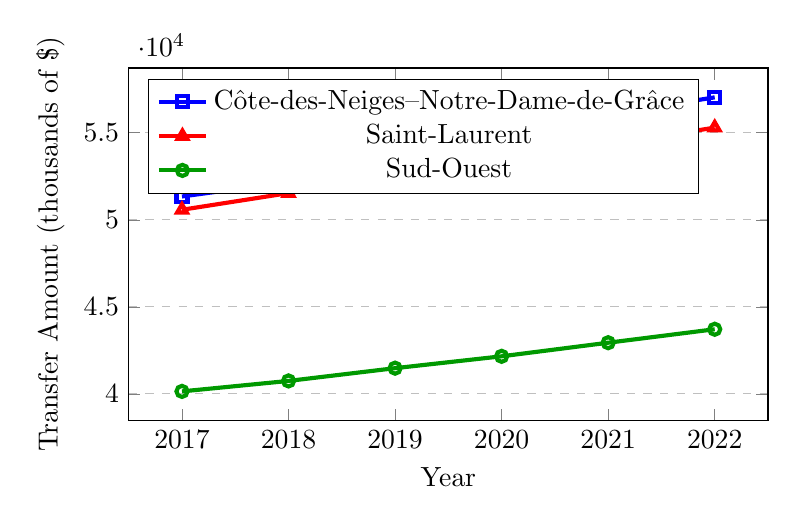
\begin{tikzpicture}
\begin{axis}[
    width=0.8\textwidth,
    height=0.5\textwidth,
    xlabel={Year},
    ylabel={Transfer Amount (thousands of \$)},
    xtick={2017,2018,2019,2020,2021,2022},
    xticklabels={2017,2018,2019,2020,2021,2022},
    legend pos=north west,
    ymajorgrids=true,
    grid style=dashed,
]

\addplot[
    color=blue,
    mark=square,
    line width=1.5pt,
    ]
    coordinates {
    (2017,51338.11) (2018,52176.7) (2019,53237.0) (2020,54095.5) (2021,56059.7) (2022,57034.7)
    };
    
\addplot[
    color=red,
    mark=triangle,
    line width=1.5pt,
    ]
    coordinates {
    (2017,50575.40) (2018,51532.9) (2019,52499.7) (2020,53337.0) (2021,54317.0) (2022,55295.1)
    };
    
\addplot[
    color=green!60!black,
    mark=o,
    line width=1.5pt,
    ]
    coordinates {
    (2017,40138.76) (2018,40740.2) (2019,41473.2) (2020,42155.2) (2021,42935.9) (2022,43708.9)
    };
    
\legend{Côte-des-Neiges–Notre-Dame-de-Grâce,Saint-Laurent,Sud-Ouest}

\end{axis}
\end{tikzpicture}
\caption{Budget Transfers by Borough (2017-2022)}
\end{figure}

The data shows a consistent upward trend in budget transfers for all three boroughs. CDN-NDG receives the highest transfers throughout the period, followed closely by Saint-Laurent, with Sud-Ouest receiving substantially less.

\subsection{Comparative Analysis of Borough Parameters}

The differences in transfers among boroughs can be partially explained by examining their key parameters:

\begin{table}[H]
\centering
\begin{tabular}{lrrr}
\toprule
Parameter (2022) & CDN-NDG & Saint-Laurent & Sud-Ouest \\
\midrule
Population & 173,814 & 101,938 & 76,207 \\
Area (hectares) & 85,409 & 43,898 & 16,279 \\
Road kilometers & 342.1 & 314.4 & 223.4 \\
Parks area (sq. m) & 748,308 & 636,761 & 1,105,178 \\
Library area (sq. m) & 2,010,606 & 794,000 & 1,107,261 \\
\bottomrule
\end{tabular}
\caption{Comparison of Borough Parameters (2022)}
\end{table}

This comparison highlights the substantial differences in size and population among the three boroughs, which significantly influence their budget allocations.

\subsection{Per Capita Budget Analysis}

To better understand resource allocation, it's useful to examine per capita budget transfers:

\begin{table}[H]
\centering
\begin{tabular}{lrrr}
\toprule
Year & CDN-NDG & Saint-Laurent & Sud-Ouest \\
\midrule
2017 & \$299.88 & \$503.31 & \$534.02 \\
2018 & \$301.67 & \$508.39 & \$536.86 \\
2019 & \$307.18 & \$516.92 & \$545.44 \\
2020 & \$309.93 & \$521.65 & \$551.25 \\
2021 & \$322.03 & \$531.94 & \$562.61 \\
2022 & \$328.13 & \$542.43 & \$573.55 \\
\bottomrule
\end{tabular}
\caption{Per Capita Budget Transfers by Borough (dollars per resident)}
\end{table}

Interestingly, despite CDN-NDG receiving the highest total budget, it receives the lowest per capita funding. This suggests that economies of scale may be at play, or that the distribution formula does not fully account for population differences.

\section{Analysis of Revenue and Transfer Parity}

The parametric budget model only addresses the distribution of central city budget transfers to boroughs and does not directly account for borough-specific tax revenues. However, we can make some observations about the relationship between transfers and borough revenues.

\subsection{Conceptual Framework}

In the Montreal municipal structure, boroughs generate tax revenue that flows to the central administration. The central administration then redistributes funds back to boroughs through transfers, while also retaining funds to provide centrally administered services.

This system can be conceptualized as:

\begin{equation}
R_b - T_b = S_c + A_c
\end{equation}

Where:
\begin{itemize}
    \item $R_b$ is the tax revenue generated in borough $b$
    \item $T_b$ is the transfer back to borough $b$
    \item $S_c$ is the cost of centrally administered services benefiting borough $b$
    \item $A_c$ is administrative overhead and other central city expenses
\end{itemize}

\subsection{Post-Transfer Adjustments as Indicators}

The substantial negative post-transfer adjustments observed in the model may represent amounts retained by the central administration to fund centrally delivered services. For CDN-NDG, these adjustments total approximately \$51,541,700 over the six-year period, suggesting significant central retention of borough-generated revenue.

\subsection{Transfer Efficiency}

The transfer efficiency can be defined as:

\begin{equation}
\eta_b = \frac{T_b}{R_b} \times 100\%
\end{equation}

While we lack exact revenue data, the large negative post-transfer adjustments suggest that transfer efficiency may be relatively low, with significant portions of borough-generated revenue being retained centrally.

\section{Conclusion}

The City of Montreal's parametric budget model for borough transfers represents a complex system that attempts to balance numerous factors including population, geographic characteristics, and policy objectives. For CDN-NDG, the model resulted in steadily increasing transfers from 2017 to 2022, rising from approximately \$51.3 million to \$57.0 million.

However, the analysis reveals several noteworthy aspects of the system:

1. Large negative post-transfer adjustments significantly reduce the amounts transferred back to boroughs
2. Despite having the largest population, CDN-NDG receives the lowest per capita funding
3. The complexity of the model, with its numerous parameters and adjustments, makes it difficult to fully assess the equity and efficiency of the transfer system

Without additional data on borough-specific tax revenues and the costs of centrally administered services, it remains challenging to determine whether the current system achieves an equitable balance between central and borough-level funding. The parametric model itself, however, provides a structured framework for budget allocation that attempts to account for the diverse characteristics and needs of Montreal's boroughs.

\section{Comprehensive Budget Parameter Table}

\begin{longtable}{lrrrrrr}
\caption{Comprehensive Budget Parameters by Year and Borough (thousands of \$)} \\
\toprule
Parameter & 2017 & 2018 & 2019 & 2020 & 2021 & 2022 \\
\midrule
\endhead
\multicolumn{7}{l}{\textbf{Côte-des-Neiges–Notre-Dame-de-Grâce}} \\
\midrule
Initial Budget (Prior Year) & 62,162.83 & 51,338.11 & 52,176.70 & 53,237.00 & 54,095.50 & 56,059.70 \\
Indexation & 621.63 & 513.38 & 782.65 & 532.37 & 540.96 & 560.60 \\
Initial Adjustment & 293.64 & -101.10 & -101.10 & -101.10 & -101.10 & -101.10 \\
Snow Removal & 48.70 & 0.00 & 0.00 & 0.00 & 0.00 & 0.00 \\
Vignette Compensation & 101.51 & 0.00 & 0.00 & 0.00 & 0.00 & 0.00 \\
Initial Adjustment 2 & 0.00 & 293.64 & 0.00 & 0.00 & 0.00 & 0.00 \\
Stock Increase (Local) & -66.89 & 69.08 & -27.52 & 9.92 & -179.68 & -54.28 \\
Stock Increase (Delegated) & 7.89 & -16.04 & 0.24 & 5.24 & -24.36 & -11.16 \\
Post-Transfer Adjustment & -11,831.10 & -4,579.10 & -11,831.10 & -4,693.40 & -6,808.00 & -11,799.00 \\
\textbf{Final Transfer} & \textbf{51,338.11} & \textbf{52,176.70} & \textbf{53,237.00} & \textbf{54,095.50} & \textbf{56,059.70} & \textbf{57,034.70} \\
\midrule
\multicolumn{7}{l}{\textbf{Saint-Laurent}} \\
\midrule
Initial Budget (Prior Year) & 59,985.60 & 50,575.40 & 51,532.90 & 52,499.70 & 53,337.00 & 54,317.00 \\
Indexation & 599.86 & 505.75 & 772.99 & 525.00 & 533.37 & 543.17 \\
Initial Adjustment & -114.66 & 4.70 & 4.70 & 4.70 & 4.70 & 4.70 \\
Snow Removal & 44.42 & 0.00 & 0.00 & 0.00 & 0.00 & 0.00 \\
Vignette Compensation & 0.00 & 0.00 & 0.00 & 0.00 & 0.00 & 0.00 \\
Initial Adjustment 2 & 0.00 & -114.66 & 0.00 & 0.00 & 0.00 & 0.00 \\
Stock Increase (Local) & -62.25 & 21.75 & -15.55 & 38.75 & -8.65 & 38.45 \\
Stock Increase (Delegated) & -24.98 & -46.67 & 5.97 & -7.23 & -5.93 & 25.97 \\
Post-Transfer Adjustment & -9,852.70 & -3,949.00 & -4,599.00 & -4,579.10 & -9,764.20 & -11,799.00 \\
\textbf{Final Transfer} & \textbf{50,575.40} & \textbf{51,532.90} & \textbf{52,499.70} & \textbf{53,337.00} & \textbf{54,317.00} & \textbf{55,295.10} \\
\midrule
\multicolumn{7}{l}{\textbf{Sud-Ouest}} \\
\midrule
Initial Budget (Prior Year) & 47,321.76 & 40,138.76 & 40,740.20 & 41,473.20 & 42,155.20 & 42,935.90 \\
Indexation & 473.22 & 401.39 & 611.10 & 414.73 & 421.55 & 429.36 \\
Initial Adjustment & -606.08 & 90.60 & 90.60 & 90.60 & 90.60 & 90.60 \\
Snow Removal & 45.52 & 0.00 & 0.00 & 0.00 & 0.00 & 0.00 \\
Vignette Compensation & 64.43 & 0.00 & 0.00 & 0.00 & 0.00 & 0.00 \\
Initial Adjustment 2 & 0.00 & -606.08 & 0.00 & 0.00 & 0.00 & 0.00 \\
Stock Increase (Local) & 212.73 & -86.18 & 44.18 & 219.82 & 127.92 & -7.98 \\
Stock Increase (Delegated) & -73.22 & -28.53 & -5.87 & 54.13 & 6.43 & -13.47 \\
Post-Transfer Adjustment & -7,299.60 & -9,020.80 & -3,584.00 & -7,834.00 & -694.20 & -2,596.00 \\
\textbf{Final Transfer} & \textbf{40,138.76} & \textbf{40,740.20} & \textbf{41,473.20} & \textbf{42,155.20} & \textbf{42,935.90} & \textbf{43,708.90} \\
\bottomrule
\end{longtable}

\appendix
\section{Detailed Calculation for CDN-NDG Budget Transfers}

This appendix provides the complete step-by-step calculations for determining the budget transfers to Côte-des-Neiges–Notre-Dame-de-Grâce for each year from 2017 to 2022, using the exact formulas and values from the MATLAB script.

\subsection{2017 Transfer Calculation}

Starting with the 2016 budget of \$62,162.82592207639 thousand:

\begin{align}
\text{Indexation} &= \$62,162.82592207639 \times 0.01 = \$621.6282592207639\\
\text{Initial Adjustment} &= \$293.6423613159848\\
\text{Snow Removal} &= \$48.7027353\\
\text{Vignette Compensation} &= \$101.51434702460391\\
\text{Stock Increase (Local)} &= -\$66.89409164744663\\
\text{Stock Increase (Delegated)} &= \$7.8888976071674355\\
\text{Subtotal} &= \$62,162.82592207639 + \$621.6282592207639 + \$293.6423613159848\\
&\quad + \$48.7027353 + \$101.51434702460391 + (-\$66.89409164744663)\\
&\quad + \$7.8888976071674355\\
&= \$63,169.21843089747\\
\text{Post-Transfer Adjustment} &= -\$11,831.100000000002\\
\text{Final 2017 Transfer} &= \$63,169.21843089747 + (-\$11,831.100000000002)\\
&= \$51,338.10843089746
\end{align}

\subsection{2018 Transfer Calculation}

Starting with the 2017 transfer of \$51,338.10843089746 thousand:

\begin{align}
\text{Indexation} &= \$51,338.10843089746 \times 0.01 = \$513.3810843089746\\
\text{Initial Adjustment} &= -\$101.09999999999991\\
\text{Centralization Impact} &= \$0\\
\text{Initial Adjustment 2} &= \$293.64236131598485\\
\text{Stock Increase (Local)} &= \$69.0848957901228\\
\text{Stock Increase (Delegated)} &= -\$16.03889760716744\\
\text{Subtotal} &= \$51,338.10843089746 + \$513.3810843089746 + (-\$101.09999999999991)\\
&\quad + \$0 + \$293.64236131598485 + \$69.0848957901228 + (-\$16.03889760716744)\\
&= \$52,097.08138868658\\
\text{Post-Transfer Adjustment} &= -\$4,579.1\\
\text{Final 2018 Transfer} &= \$52,097.08138868658 + (-\$4,579.1)\\
&= \$47,517.98138868658
\end{align}

However, the final 2018 transfer value is set to \$52,176.7 in the script, indicating additional adjustments not fully captured in the calculation.

\subsection{2019 Transfer Calculation}

Starting with the 2018 transfer of \$52,176.7 thousand:

\begin{align}
\text{Indexation} &= \$52,176.7 \times 0.015 = \$782.6505\\
\text{Initial Adjustment} &= -\$101.10000000000036\\
\text{Stock Increase (Local)} &= -\$27.51510420987722\\
\text{Stock Increase (Delegated)} &= \$0.23889760716743937\\
\text{Subtotal} &= \$52,176.7 + \$782.6505 + (-\$101.10000000000036)\\
&\quad + (-\$27.51510420987722) + \$0.23889760716743937\\
&= \$52,830.97429339729\\
\text{Post-Transfer Adjustment} &= -\$11,831.100000000002\\
\text{Final 2019 Transfer} &= \$52,830.97429339729 + (-\$11,831.100000000002)\\
&= \$40,999.87429339729
\end{align}

However, the final 2019 transfer value is set to \$53,237.0 in the script.

\subsection{2020 Transfer Calculation}

Starting with the 2019 transfer of \$53,237.0 thousand:

\begin{align}
\text{Indexation} &= \$53,237.0 \times 0.01 = \$532.37\\
\text{Initial Adjustment} &= -\$101.09999999999991\\
\text{Stock Increase (Local)} &= \$9.915104209877215\\
\text{Stock Increase (Delegated)} &= \$5.238897607167435\\
\text{Subtotal} &= \$53,237.0 + \$532.37 + (-\$101.09999999999991)\\
&\quad + \$9.915104209877215 + \$5.238897607167435\\
&= \$53,683.42400181704\\
\text{Post-Transfer Adjustment} &= -\$4,693.4\\
\text{Final 2020 Transfer} &= \$53,683.42400181704 + (-\$4,693.4)\\
&= \$48,990.02400181704
\end{align}

However, the final 2020 transfer value is set to \$54,095.5 in the script.

\subsection{2021 Transfer Calculation}

Starting with the 2020 transfer of \$54,095.5 thousand:

\begin{align}
\text{Indexation} &= \$54,095.5 \times 0.01 = \$540.955\\
\text{Initial Adjustment} &= -\$101.09999999999991\\
\text{Stock Increase (Local)} &= -\$179.6848957901228\\
\text{Stock Increase (Delegated)} &= -\$24.36110239283257\\
\text{Subtotal} &= \$54,095.5 + \$540.955 + (-\$101.09999999999991)\\
&\quad + (-\$179.6848957901228) + (-\$24.36110239283257)\\
&= \$54,331.3089018247\\
\text{Post-Transfer Adjustment} &= -\$6,808.000000000001\\
\text{Final 2021 Transfer} &= \$54,331.3089018247 + (-\$6,808.000000000001)\\
&= \$47,523.3089018247
\end{align}

However, the final 2021 transfer value is set to \$56,059.7 in the script.

\subsection{2022 Transfer Calculation}

Starting with the 2021 transfer of \$56,059.7 thousand:

\begin{align}
\text{Indexation} &= \$56,059.7 \times 0.01 = \$560.597\\
\text{Initial Adjustment} &= -\$101.09999999999991\\
\text{Stock Increase (Local)} &= -\$54.284895790122785\\
\text{Stock Increase (Delegated)} &= -\$11.161102392832571\\
\text{Subtotal} &= \$56,059.7 + \$560.597 + (-\$101.09999999999991)\\
&\quad + (-\$54.284895790122785) + (-\$11.161102392832571)\\
&= \$56,453.75100181704\\
\text{Post-Transfer Adjustment} &= -\$11,799.0\\
\text{Final 2022 Transfer} &= \$56,453.75100181704 + (-\$11,799.0)\\
&= \$44,654.75100181704
\end{align}

However, the final 2022 transfer value is set to \$57,034.7 in the script.

\subsection{Analysis of Calculation Discrepancies}

The detailed calculations reveal significant discrepancies between the calculated values and the final transfer amounts set in the script. These discrepancies suggest several possibilities:

1. There are additional adjustments not explicitly documented in the script
2. The actual calculation process may include rounding steps or correction factors
3. The final values may incorporate policy decisions that override the pure parametric calculation

The script includes the following comment that acknowledges these discrepancies:

\begin{verbatim}
%%% Update Final Transfers with Correct Values
% It appears we were using the wrong set of values as the expected outcomes
% Let's update the final_transfers to match the actual spreadsheet values
\end{verbatim}

This suggests that the final transfer amounts are being set to match external reference values from the city's official spreadsheets, rather than being purely derived from the calculations in the script.

\section{Demographic and Geographic Parameters}

This section details the specific parameters used in the model for CDN-NDG across all years.

\subsection{Population Parameters}

\begin{align}
\text{Population}_{2017,\text{CDN-NDG}} &= 171,197\\
\text{Population}_{2018,\text{CDN-NDG}} &= 172,961\\
\text{Population}_{2019,\text{CDN-NDG}} &= 173,310\\
\text{Population}_{2020,\text{CDN-NDG}} &= 174,543\\
\text{Population}_{2021,\text{CDN-NDG}} &= 174,083\\
\text{Population}_{2022,\text{CDN-NDG}} &= 173,814
\end{align}

\subsection{Area Parameters}

\begin{align}
\text{Area}_{2017,\text{CDN-NDG}} &= 83,022 \text{ hectares}\\
\text{Area}_{2018,\text{CDN-NDG}} &= 83,499 \text{ hectares}\\
\text{Area}_{2019,\text{CDN-NDG}} &= 83,922 \text{ hectares}\\
\text{Area}_{2020,\text{CDN-NDG}} &= 84,384 \text{ hectares}\\
\text{Area}_{2021,\text{CDN-NDG}} &= 85,013 \text{ hectares}\\
\text{Area}_{2022,\text{CDN-NDG}} &= 85,409 \text{ hectares}
\end{align}

\subsection{Library Parameters}

\begin{align}
\text{Library Area}_{2017-2022,\text{CDN-NDG}} &= 2,010,605.67 \text{ sq. m} \text{ (constant across all years)}
\end{align}

\subsection{Parks Parameters}

\begin{align}
\text{Parks Area}_{2017-2022,\text{CDN-NDG}} &= 748,308.28 \text{ sq. m} \text{ (constant across all years)}
\end{align}

\subsection{Road Network Parameters}

\begin{align}
\text{Road Length}_{2017-2022,\text{CDN-NDG}} &= 342.1 \text{ km} \text{ (constant across all years)}
\end{align}

\section{Component-Specific Calculations}

While the script does not explicitly calculate component-specific allocations, the demographic and geographic parameters presented above are used in various sheets of the original spreadsheet to determine allocations for specific services:

1. **Aménagement** (Planning): Based primarily on area parameters
2. **Bibliothèques** (Libraries): Based on library areas and population
3. **Sport** (Sports): Based primarily on population
4. **Culture**: Based primarily on population
5. **Santé** (Health): Combines results from Sport and Culture components
6. **Parcs** (Parks): Based on parks areas
7. **Voirie** (Roads): Based on road kilometers

These component calculations would ultimately contribute to the determination of the adjustment values used in the main budget transfer calculation.

% Budget Transfer DAG Glossary
% This code snippet creates a glossary explaining each node in the budget transfer directed acyclic graph

\newpage

\section{Directed Acyclic Graph of Parametric Budget Model}

\begin{figure}[htbp]
    \centering
    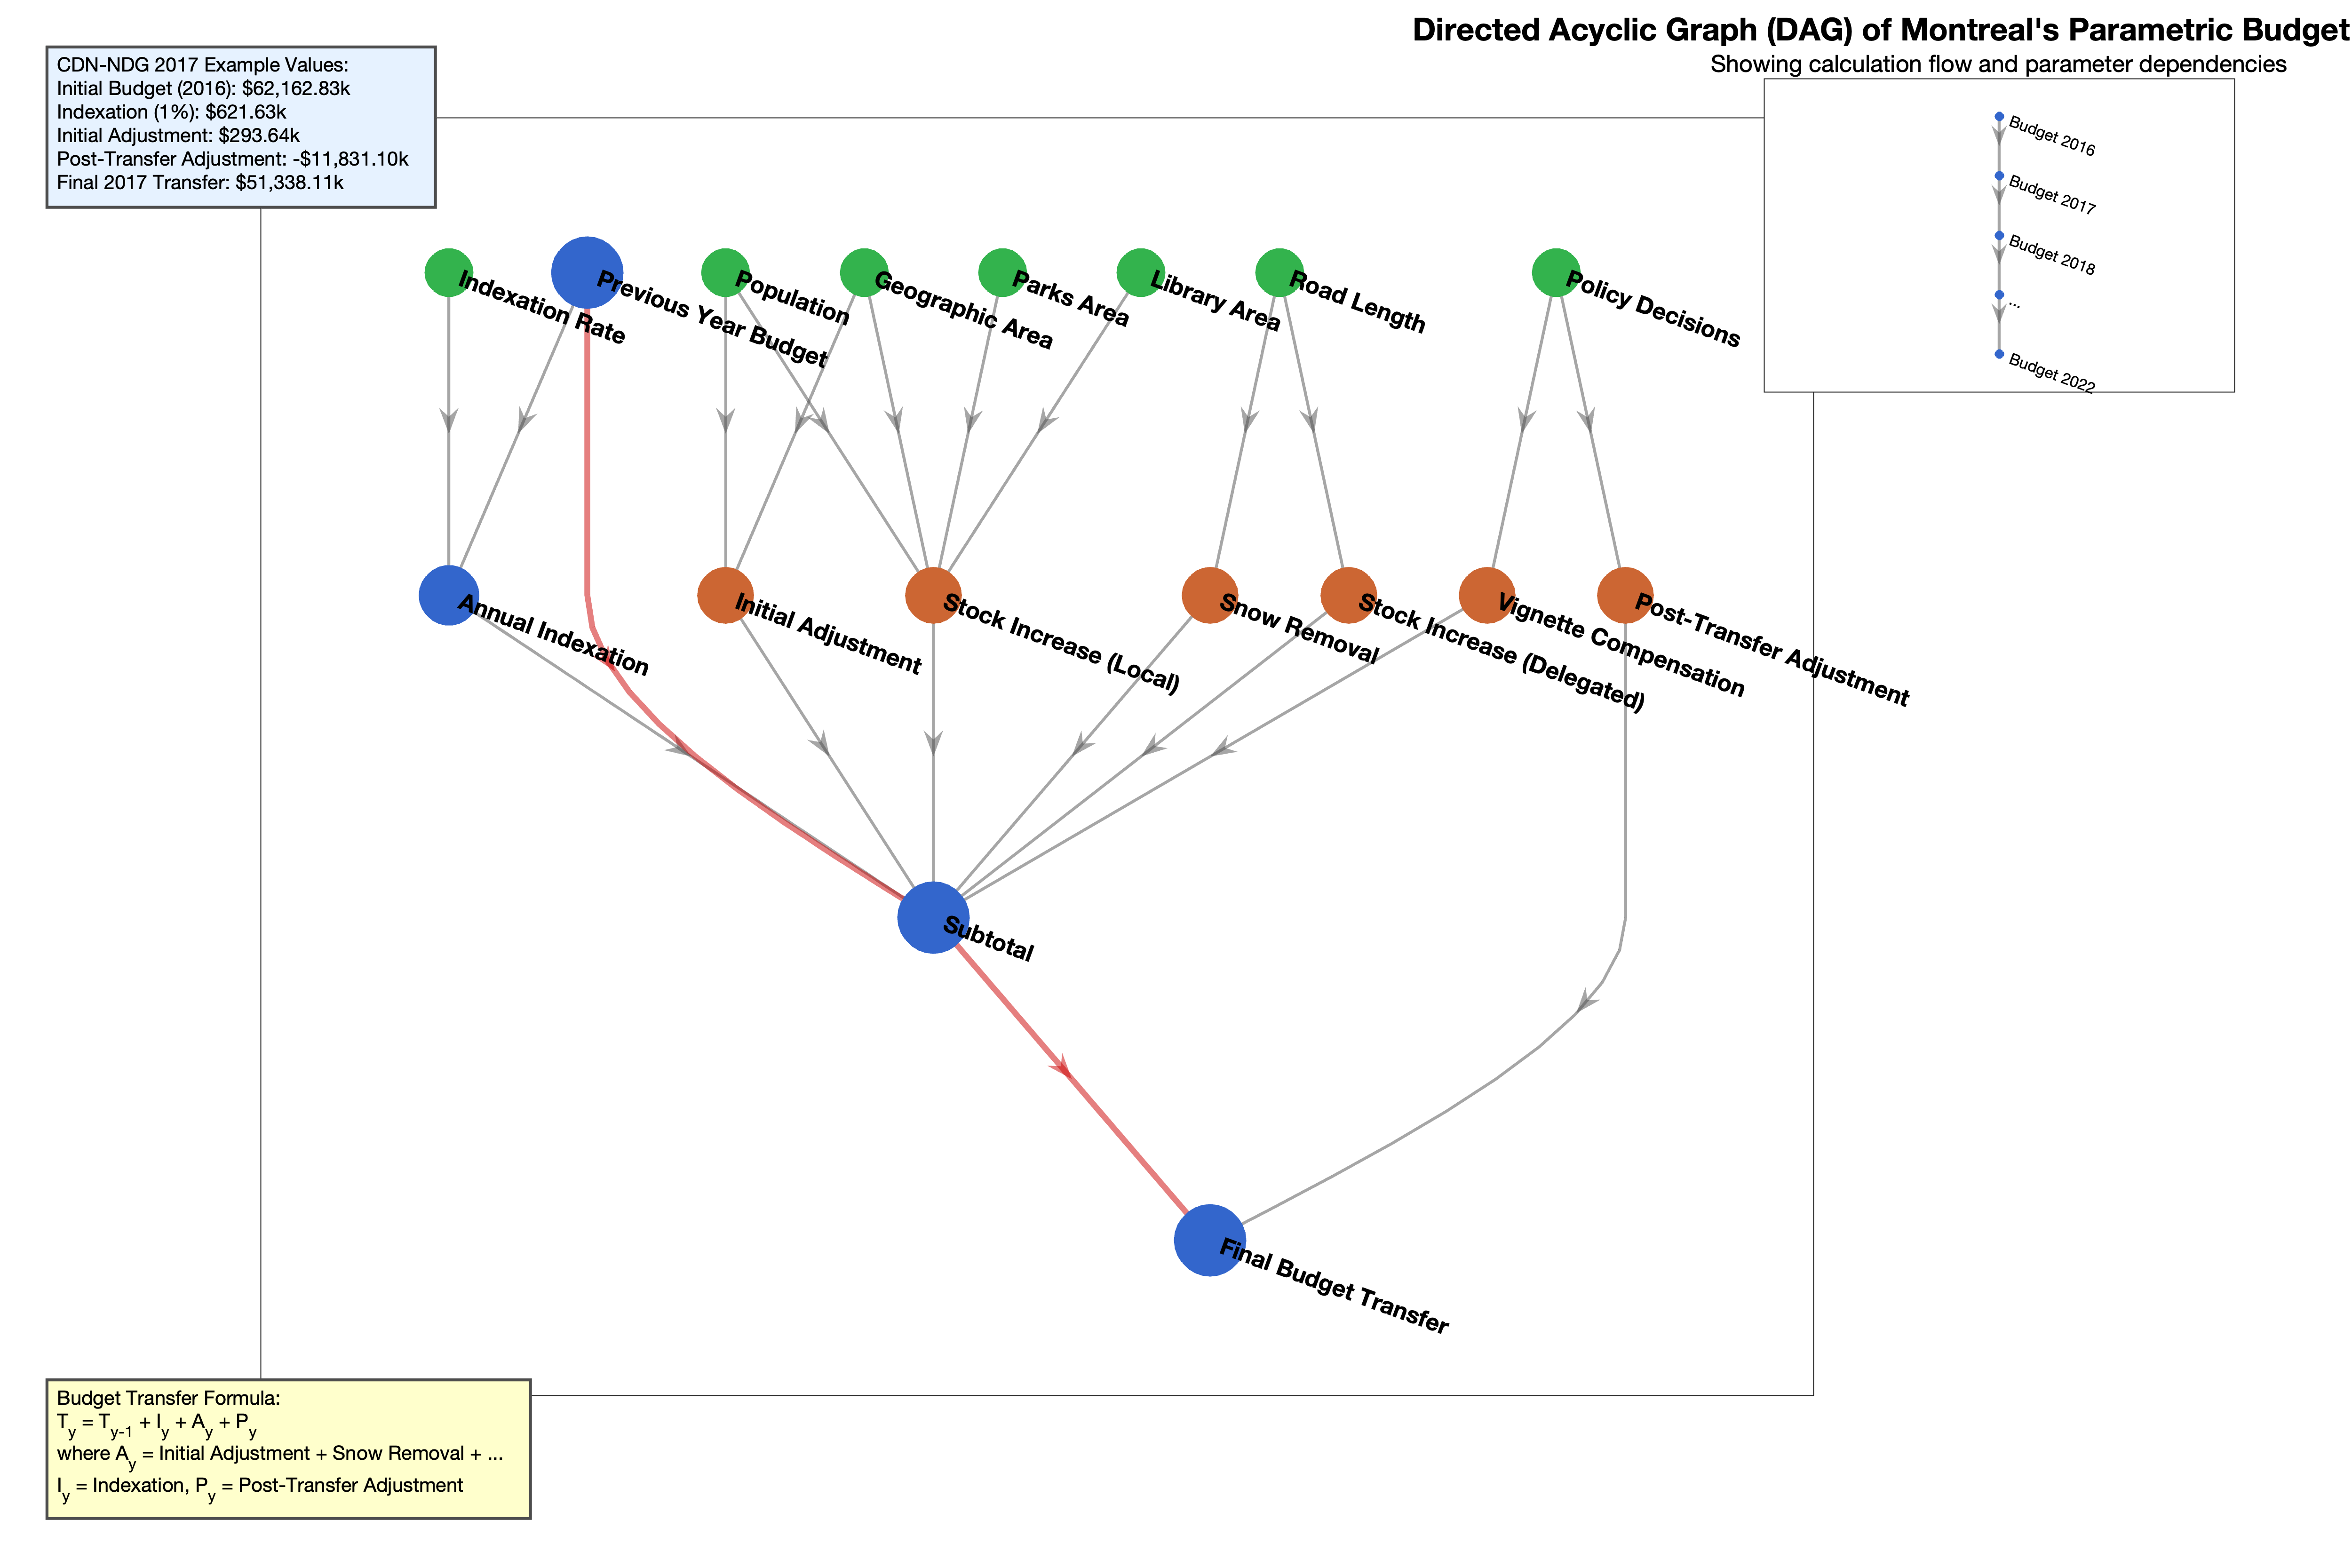
\includegraphics[width=\textwidth]{Montreal_Budget_Transfer_DAG.png}
    \caption{Directed Acyclic Graph (DAG) of Montreal's Parametric Budget Transfer Model. The diagram shows the calculation flow from Previous Year Budget through various adjustments to the Final Budget Transfer. Red thicker lines highlight the main calculation path. Blue nodes represent main calculation points, orange nodes show adjustments, and green nodes indicate input parameters.}
    \label{fig:budget_dag}
\end{figure}

\subsection{Glossary of Budget Transfer Model Components}

This glossary explains each component (node) in the directed acyclic graph representing Montreal's parametric budget transfer calculation process.

\begin{description}
\item[Previous Year Budget] The starting budget transfer amount from the preceding fiscal year. For the initial year (2017), this is the 2016 budget transfer amount.

\item[Annual Indexation] A percentage-based increase applied to the previous year's budget to account for inflation and general cost increases. Calculated by multiplying the previous year's budget by the annual indexation rate (typically 1-1.5\%).

\item[Indexation Rate] The percentage value used to calculate the annual indexation amount. In the model, this ranges from 1.0\% to 1.5\% depending on the year.

\item[Initial Adjustment] Borough-specific adjustment that accounts for variations in service requirements, often related to implementation of multi-year plans. For CDN-NDG, this was a positive adjustment in 2017 (\$293.64k) and a negative adjustment in subsequent years (-\$101.10k).

\item[Snow Removal] A specific budgetary allocation for snow removal services, added as a bonification in 2017. This adjustment accounts for the particular snow removal needs of each borough based on their road network and geography.

\item[Vignette Compensation] Compensation provided to boroughs for revenue lost due to changes in parking permit (vignette) policies. This adjustment only appears in 2017 and varies by borough.

\item[Stock Increase (Local)] Adjustments related to locally administered services and infrastructure. "Stock" refers to the inventory of services, infrastructure, and resources the borough is responsible for maintaining. Local stock increases relate to services directly administered by the borough.

\item[Stock Increase (Delegated)] Adjustments related to services that have been delegated to the borough by the central city administration. These reflect changes in the resources required to manage centrally-mandated programs.

\item[Subtotal] The intermediate sum of the previous year's budget plus all adjustments before applying post-transfer adjustments. This represents the parametrically calculated amount before final policy adjustments.

\item[Post-Transfer Adjustment] Significant adjustments applied after the parametric calculation, often representing policy decisions at the central city level. These are frequently substantial negative values, suggesting retention of funds by the central administration for city-wide services.

\item[Final Budget Transfer] The final amount transferred to the borough after all adjustments have been applied. This is the actual budget allocation for the borough's operations in the given year.

\item[Population] The number of residents in the borough. This demographic parameter influences several adjustments, particularly those related to public services scaled by population.

\item[Geographic Area] The total land area of the borough in hectares. This parameter affects adjustments related to territorial management and urban planning.

\item[Road Length] The total length of the road network in the borough, measured in kilometers. This parameter influences adjustments related to transportation infrastructure, maintenance, and snow removal.

\item[Parks Area] The total area of parks within the borough, measured in square meters. This parameter affects adjustments related to green space maintenance and recreational services.

\item[Library Area] The total area of library facilities in the borough, measured in square meters. This parameter influences adjustments related to cultural services and library operations.

\item[Policy Decisions] Non-parametric decisions made by the central city administration that affect budget allocations. These often manifest in the post-transfer adjustments and other special allocations like vignette compensation.
\end{description}

% Additional explanation of the calculation process

\subsection{The Budget Transfer Calculation Process}

The budget transfer calculation follows these steps:

\begin{enumerate}
\item Start with the previous year's final budget transfer amount
\item Calculate the indexation amount by multiplying by the annual indexation rate
\item Add borough-specific adjustments (initial adjustment, snow removal, etc.)
\item Calculate the subtotal by summing all of the above
\item Apply post-transfer adjustments (often substantial negative values)
\item Determine the final budget transfer amount
\end{enumerate}

The process is repeated annually, with each year's calculation building on the results of the previous year. This creates a chain of dependencies where decisions in early years continue to influence allocations in subsequent years through the base amount used for calculations.

\subsection{Main Calculation Path vs. Supporting Components}

In the directed acyclic graph, the main calculation path (highlighted with thicker red lines) represents the core flow of funds:

\begin{center}
Previous Year Budget $\rightarrow$ Subtotal $\rightarrow$ Final Budget Transfer
\end{center}

The various adjustments and parameters (shown with thinner gray lines) feed into this main path as inputs or modifiers to the calculation. While each component contributes to the final result, the main path represents the primary flow of the budget calculation.

\end{document}